\section{Evaluations}
\label{sec:eval}

\begin{figure}
  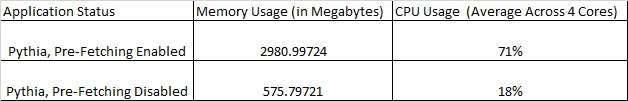
\includegraphics[width=\linewidth]{applicationResourceUsageTable1.jpg}
  \caption{A Table depicting the Main memory and CPU Usage of Our Application with Prefetching enabled and disabled.}
  \label{fig:table1}
\end{figure}

\begin{figure}
  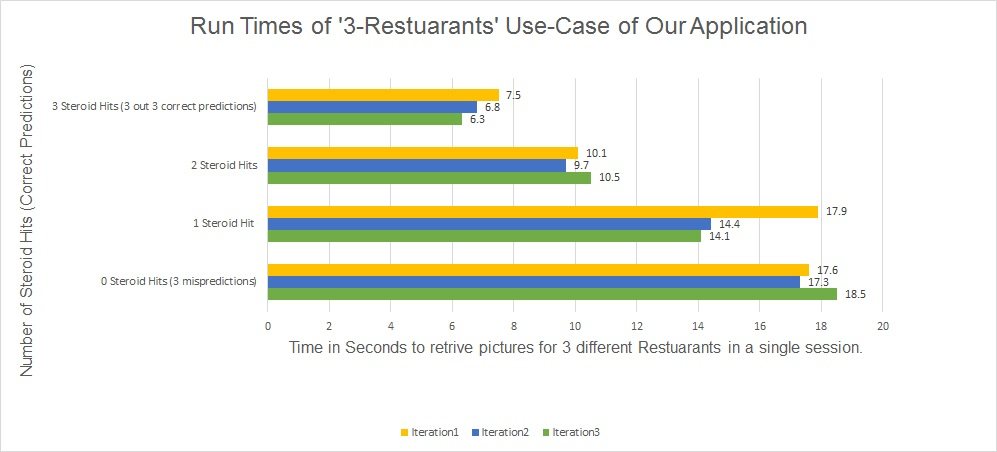
\includegraphics[width=\linewidth]{runTimeChart1.jpg}
  \caption{A Graph depicting runtimes of our Application clustered by Number of Steroid Hits (Correct Predictions).}
  \label{fig:graph1}
\end{figure}


Our evaluation answers two key questions about our system:
\begin{itemize}
\item How much does Pythia speed up the user perceived latency? (In the best case scenario? And in the worst case?)
\item How many excess resources does our implemented system consume? (Is the resource-consumption trade-off worth the speed up?)
\end{itemize}

We used a single Lenovo and IBM Thinkpad x220 for the client machine for running the implemented application. The Thinkpad personal computer has a 'Intel® Core™ i5-2520M (2.5GHz, 3MB L3 cache)', 16GB of DRAM, and a 240 GB solid state hard drive. The machine has a 'ThinkPad 11b/g/n Wireless LAN Mini-PCI Express Adapter II' network adapter. We run the application 12 times on Ubuntu version 14.04.5 LTS with kernel version 3.19. We ran the experiment in two different configurations, one with prefetching enabled and the other with prefetching turned off. The table in Figure 1 shows that disabling the prefetching feature significantly reduces both the memory usage and the CPU usage of our program. In other words, the implemented speculative execution system captures and uses the excess RAM and CPU cycles that would have otherwise been wasted while the user was thinking. Turning off the speculation feature reduces memory usage from almost 3 Gigabytes to a little over one-half of a gigabyte. Likewise for CPU Usage, the Average CPU load across 4 cores is reduced by a factor of almost 4; from 71 percent usage to 18 percent processor usage.

Figure 2 illustrates the relationship between number of accurate predictions and user-perceived response latency for our application. In the 3 cases where all Steroids hit, (in other words, that our application correctly predicted and prefetched the images for all 3 of the 3 restaurants the user explored) the user's session gets sped up from a 17.6, 17.3, and 18.5 second run-time to 7.5, 6.8, and 6.3 second run-times respectively. This is a significant speed up! Our speculative execution system speeds up the user's session by an order of magnitude, specifically improving the user-experience with our application as an interactive session. In the Worst case, where all of our Steroids miss (In other words, all of predictions were wrong and the prefetched data is not used) we simply fetch at request time, and thus deliver latency similar to the case where speculation is turned off. So at best we save 10 seconds in a traditionally 18-second user session, and at worst we take 18 seconds in a traditionally 18-second user session. 
